As discussed in the previous section there are several issues with the first iteration the second iteration aims to solve. Most of the improvements over the first iteration are not seen by the end-user as the bulk of the improvement is the code handling the musical objects. 

\section{Software architecture}
Figure~\ref{fig:iter2_architecture} shows the second iteration in the same architectural style as the other iterations. Compared with the first iteration, the generation now passes through explicit musical objects such as \texttt{Motif}, \texttt{Bar}, and \texttt{Phrase}, and the generator reuses motivic material instead of producing every event independently.

\begin{figure}[htbp]
  \centering
  \resizebox{\textwidth}{!}{%
  \begin{tikzpicture}[
    >=Latex,
    font=\small,
    node distance=8mm and 10mm,
    stage/.style={
      draw,
      rounded corners=3pt,
      align=center,
      minimum width=0.42\textwidth,
      minimum height=10mm,
      fill=gray!8
    },
    support/.style={
      draw,
      rounded corners=3pt,
      align=center,
      minimum width=0.24\textwidth,
      minimum height=9mm,
      fill=blue!6
    },
    output/.style={
      draw,
      rounded corners=3pt,
      align=center,
      minimum width=0.24\textwidth,
      minimum height=9mm,
      fill=green!8
    },
    arrow/.style={
      -{Latex[length=2.3mm]},
      thick
    }
  ]

    \node[stage] (input) {User input and fixed script values\\key, bars, allowed beat values};
    \node[stage, below=of input] (main) {\texttt{main.py}\\requests a phrase, then triggers LilyPond export and playback};
    \node[stage, below=of main] (generator) {\texttt{generators.py}\\motif creation, phrase generation,\\bar filling and tonic ending};
    \node[stage, below=of generator] (phrase) {\texttt{Motif}, \texttt{Bar}, and \texttt{Phrase}\\more explicit musical object model};
    \node[stage, below=of phrase] (render) {\texttt{lilypond.py}\\single-staff LilyPond export, PDF generation,\\and audio rendering};

    \node[support, left=18mm of generator] (music) {\texttt{music.py}\\note classes, key handling,\\and pitch conversion};
    \node[support, right=18mm of generator] (constraints) {\texttt{constraints.py}\\valid scale notes and small-step\\interval restrictions};

    \node[output, below left=10mm and 10mm of render] (ly) {\texttt{.ly} source};
    \node[output, below=10mm of render] (pdf) {cropped \texttt{.pdf}};
    \node[output, below right=10mm and 10mm of render] (audio) {\texttt{.midi} and \texttt{.wav}};

    \draw[arrow] (input) -- (main);
    \draw[arrow] (main) -- (generator);
    \draw[arrow] (generator) -- (phrase);
    \draw[arrow] (phrase) -- (render);

    \draw[arrow] (music.east) -- (generator.west);
    \draw[arrow] (constraints.west) -- (generator.east);

    \draw[arrow] (render) -- (ly);
    \draw[arrow] (render) -- (pdf);
    \draw[arrow] (render) -- (audio);

  \end{tikzpicture}%
  }
  \caption{Architecture of the second iteration melody generator. Motivic material and phrase-level objects make the generator more structured than the first iteration, even though the constraint handling is still lightweight and local.}\label{fig:iter2_architecture}
\end{figure}

\section{Implementation}
As mentioned the code structure has been improved in this iteration, below you can see an excerpt form the code in the \textit{music.py} file.
\lstinputlisting[language=Python, firstline=22, lastline=49]{../../code/.old/.old_iter2/music.py}
Comparing to the first iteration this has a more defined structure and easier to read, however it needs improvement.

The second iteration improved upon the structure of the melody. By using a motif we forced some self-similarity in the generated melody which helped generating something more musical, however this generation is very dependent on the generated motif being musical. 

Structurally the second iteration is quite similar to the first iteration however, the objects used for handling the melodies and such are more robust and easier to understand. However they are not in a final state where we will re-use it in its entirety for the next iteration. 

\section{Results}
We can see in Example~\ref{fig:iter2_melody} that we have a more defined structure. The generator works by generating a motif which is then re-used in every measure in the piece. The rest of the measures are filled with random notes moving by 2nds or 3rds to make a somewhat coherent and singable melody.

\begin{example}
  \begin{center}
    
\includegraphics[width=0.95\textwidth]{examples/iter2/melody.cropped.pdf}
  \end{center}
  \caption{Demonstration of a melody generated using the second iteration. \examplelink.}\label{fig:iter2_melody}
\end{example}

\begin{example}
  \begin{center}
    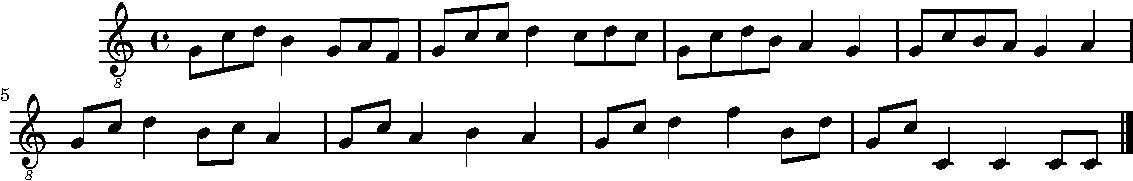
\includegraphics[width=0.95\textwidth]{examples/iter2/melody_alt1.cropped.pdf}
  \end{center}
  \caption{A second generated melody from the second iteration, showing the same motif-reuse strategy with a different random outcome. \examplelink.}\label{fig:iter2_melody_alt1}
\end{example}

\begin{example}
  \begin{center}
    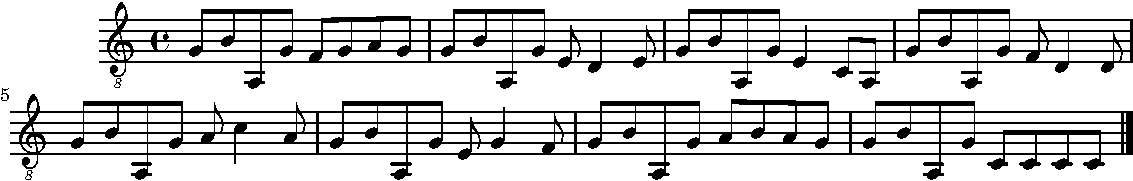
\includegraphics[width=0.95\textwidth]{examples/iter2/melody_alt2.cropped.pdf}
  \end{center}
  \caption{A third generated melody from the second iteration, again reusing an initial motif across the phrase. \examplelink.}\label{fig:iter2_melody_alt2}
\end{example}

\begin{example}
  \begin{center}
    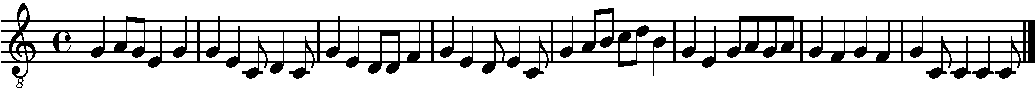
\includegraphics[width=0.95\textwidth]{examples/iter2/melody_alt3.cropped.pdf}
  \end{center}
  \caption{A fourth generated melody from the second iteration, illustrating how the same method can still lead to noticeably different melodic surfaces. \examplelink.}\label{fig:iter2_melody_alt3}
\end{example}

The generated melodies are still quite random and does not follow any musical form or adhere to melodic restrictions other than that the melody has smaller steps and not big leaps. 

\section{Discussion}
The most glaring issue with this iteration is that the melodic rules have not been formalized and implemented as code. Generating a melody using this restricted form of generation works well when the generated motif is good, and with the current implementation this only happens randomly. By implementing melodic rules and restrictions this generator will greatly improve the melody generation.

In the first iteration also had the ability to generate several voices at the same time, however, this will not be re-implemented until the melodic generation has been improved and we can enforce harmonic restrictions on one voice. If this is achieved then multi-voice generation will become much more interesting. 

Additionally the second iteration does not properly spell all notes in the different keys, this does not affect the generation in any way, though it is a trivial fix it was not implemented since the structure of the second iteration was incompatible with it. Therefore it will only be implemented in the final iteration.

We would also like to implement augmentation of a given melody or phrase, meaning the ability to transpose it up or down or use the same rhythmic outline and moving the notes around to follow a new chord. This will help develop the generated motif and melody to follow a more structured outline of a well composed melody. A key to a good melody is self-similarity, the second iteration just has repetition of a motif, not variations of it. \\


\noindent
The main goals of the third iteration is to be able to augment already generated melodies and be able to enforce constraints on the generation. To ble able to easily augment the melodies and phrases we need a robust model for the melodies made of good objects. Well designed objects is also key to ble able to enforce constraints.
